%% The first command in your LaTeX source must be the \documentclass command.
\documentclass[acmconf]{acmart}
% % Packages
%\usepackage{cite}
\usepackage{listings}
\usepackage{amsmath,amssymb,amsfonts}
\usepackage{algorithmic}
\usepackage{graphicx}
\usepackage{textcomp}
\usepackage{xcolor}
\usepackage{booktabs}
\usepackage{parskip}
\setlength{\parskip}{1em}
\usepackage[bottom]{footmisc}
\usepackage{url}
\usepackage{enumitem}
\usepackage{hyperref}
\usepackage{totpages}

%% \BibTeX command to typeset BibTeX logo in the docs
\AtBeginDocument{%
  \providecommand\BibTeX{{%
    \normalfont B\kern-0.5em{\scshape i\kern-0.25em b}\kern-0.8em\TeX}}}

%% Rights management information.  This information is sent to you
%% when you complete the rights form.  These commands have SAMPLE
%% values in them; it is your responsibility as an author to replace
%% the commands and values with those provided to you when you
%% complete the rights form.
% \setcopyright{acmcopyright}
% \copyrightyear{2018}
% \acmYear{2018}
% \acmDOI{10.1145/1122445.1122456}

% %% These commands are for a PROCEEDINGS abstract or paper.
% \acmConference[Woodstock '18]{Woodstock '18: ACM Symposium on Neural
%   Gaze Detection}{June 03--05, 2018}{Woodstock, NY}
% \acmBooktitle{Woodstock '18: ACM Symposium on Neural Gaze Detection,
%   June 03--05, 2018, Woodstock, NY}
% \acmPrice{15.00}
% \acmISBN{978-1-4503-XXXX-X/18/06}



%%
%% The majority of ACM publications use numbered citations and
%% references.  The command \citestyle{authoryear} switches to the
%% "author year" style.
%%
%% If you are preparing content for an event
%% sponsored by ACM SIGGRAPH, you must use the "author year" style of
%% citations and references.
%% Uncommenting
%% the next command will enable that style.
%%\citestyle{acmauthoryear}

%%
%% end of the preamble, start of the body of the document source.
\begin{document}

% Specify path to images
\graphicspath{ {./img/} }

% import custom commands found in commands.tex
\newcommand{\fix}[1]{\textcolor{red}{#1}}
\newcommand{\derek}[1] {\textcolor{blue}{\textbf{[Derek: #1]}}}
\newcommand{\neha}[1] {\textcolor{green}{\textbf{[Neha: #1]}}}
\newcommand{\keanu}[1] {\textcolor{orange}{\textbf{[Keanu: #1]}}}
\newcommand{\manish}[1] {\textcolor{cyan}{\textbf{[Manish: #1]}}}
% set up commands to format RQ nicely
\newlist{questions}{enumerate}{2}
\setlist[questions,1]{label=RQ\arabic*.,ref=RQ\arabic*}
\setlist[questions,2]{label=(\alph*),ref=\thequestionsi(\alph*)}

%%
%% The "title" command has an optional parameter,
%% allowing the author to define a "short title" to be used in page headers.
\title[Survival Analysis of Open Source Projects]{Two Differing Approaches to Survival Analysis of Open Source Python Projects}

%%
%% The "author" command and its associated commands are used to define
%% the authors and their affiliations.
\author{Derek Robinson}
\email{drobinson@uvic.ca}
\author{Keanelek Enns}
\email{keanelekenns@uvic.ca}
\author{Neha Koulecar}
\email{nehakoulecar@uvic.ca}
\author{Manish Sihag}
\email{manishsihag@uvic.ca}
\affiliation{%
  \institution{\\University of Victoria}
  \department{Computer Science}
  \streetaddress{PO Box 1700 STN CSC}
  \city{Victoria}
  \state{British Columbia}
  \country{Canada}
  \postcode{V8W 2Y2}
}

%%
%% By default, the full list of authors will be used in the page
%% headers. Often, this list is too long, and will overlap
%% other information printed in the page headers. This command allows
%% the author to define a more concise list
%% of authors' names for this purpose.
\renewcommand{\shortauthors}{D. Robinson, K. Enns, N. Koulecar, M. Sihag}

%%
%% The abstract is a short summary of the work to be presented in the
%% article.
\begin{abstract}
\keanu{Abstract Pending}
\end{abstract}

%%
%% The code below is generated by the tool at http://dl.acm.org/ccs.cfm.
%%
\begin{CCSXML}
<ccs2012>
<concept>
<concept_id>10011007.10011074.10011134.10003559</concept_id>
<concept_desc>Software and its engineering~Open source model</concept_desc>
<concept_significance>500</concept_significance>
</concept>
<concept>
<concept_id>10002951.10003227.10003351</concept_id>
<concept_desc>Information systems~Data mining</concept_desc>
<concept_significance>300</concept_significance>
</concept>
</ccs2012>
\end{CCSXML}

\ccsdesc[500]{Software and its engineering~Open source model}
\ccsdesc[300]{Information systems~Data mining}

%%
%% Keywords. The author(s) should pick words that accurately describe
%% the work being presented. Separate the keywords with commas.
\keywords{data science, survival analysis, open source, python, Kaplan Meier, Cox proportional hazards model, Bayesian analysis}


%%
%% This command processes the author and affiliation and title
%% information and builds the first part of the formatted document.
\maketitle

\section{Introduction}
The developers of Open Source Software (OSS) projects are often part of decentralized and geographically distributed teams of volunteers.
As these developers volunteer their free time to build such OSS projects, they likely want to be confident that the projects they work on will not become inactive.
If OSS developers are aware of key attributes that are associated with long-lasting projects, they can make informed assessments of a given project before devoting their time to it or they can strive to make their own projects exhibit those attributes.
Understanding which attributes of an OSS project lead to its longevity is what motivated Ali \emph{et al.} to apply survival analysis techniques commonly found in biostatistics to study the probability of survival for popular OSS Python projects \cite{ali2020cheating}.
Ali \emph{et al.} specifically studied the effect of the following attributes on the survival of OSS Python projects: publishing major releases, the use of multiple hosting services, the type of version control system (VCS), and the size of the volunteer team.

Survival analysis is a set of methods used to determine how long an entity will live (or the time to a given event) and is most often used in the medical field.
\keanu{do we need to find a citation for this claim/definition?}
For example, survival analysis techniques can determine the probability that a patient will survive when given a certain treatment. 
Ali \emph{et al.} use a frequentist approach to survival analysis with methods including the Kaplan-Meier (K-M) survival estimator and the Cox Proportional-Hazards model.
Though there are advantages to using such approaches \keanu{list some advantages and cite}, another approach to survival analysis, Bayesian analysis, has its own set of advantages, namely \keanu{find the advantages, list them, cite}.

The authors of this paper resonate with Ali \emph{et al.'s} motivation. 
This paper serves as a replication of their paper \cite{ali2020cheating} (referred to as the original paper from here on)  and seeks to determine if there are gaps or shortcomings in their analysis.
This replication also provides artifacts so that others may see how the study was conducted and reproduce it with ease.
For the sake of the authors' curiousity, an additional attribute of the data was analyzed: the commit frequency of the project.
In addition to the replication, this paper analyzes the same data set using a Bayesian approach to survival analysis as outlined in \cite{kelter2020bayesian} and seeks to compare the results of frequentist and Bayesian approaches in the same domain.
Thus, the research questions this paper answers are as follows:

\begin{questions}
    \item How do major releases, the use of multiple hosting services, the type of VCS, and the size of the volunteer team affect the probability of survival of an OSS Python project?
    \item How does the commit frequency of an OSS Python project affect the probability of it's survival?
    \item How do the findings of frequentist survival analysis differ from Bayesian survival analysis?
\end{questions}

The following section describes the data used for the studies in this paper. Section 3 covers the methods used for the replication, additional frequentist analysis, and Bayesian analysis studies.
Section 4 shows the results for each analysis.
Section 5 is a discussion about the limitations of the study, the differences between the types of analysis performed, and suggestions about future work in the topic.
The final section concludes by summarizing the purpose and findings of this paper. 

\section{Data}

Performing survival analysis of OSS projects requires a data set that records the repositories for projects on common VCSs, including a history of all commits (revisions from here on out) and major releases (revisions of note, often with a specific name and release date) \cite{ali2020cheating}.
Revisions are used to assess the activity or health of a project.
The assumption of the original paper was that revisions, no matter how far apart, indicate a healthy project.

The \emph{popular-3k-python} subset of the Software Heritage graph data set \cite{pietri2019software} was used in both the original paper and this paper.
This data set \keanu{Doing a little bit of searching, it appears that dataset is more of a jargon term, so maybe we should try to stick with data set.} contains information on roughly 3000 popular Python projects hosted on GitHub/GitLab, Debian, and PyPI between 2005 and 2018.
The Software Heritage Graph offers a tutorial on how to import this data \cite{SQLdataset} as well as an explanation of the structure of the data set (a database schema can be seen in figure 2 of their document) \cite{pietri2019software}.

Most of the analyzed features or attributes of the projects in the original study are not present in the raw data set; data manipulation was required in order to calculate and extract the desired attributes of the projects.

% If we want filler we can add the schema diagram and talk about it.
% \begin{figure}[h]
% \centering
% 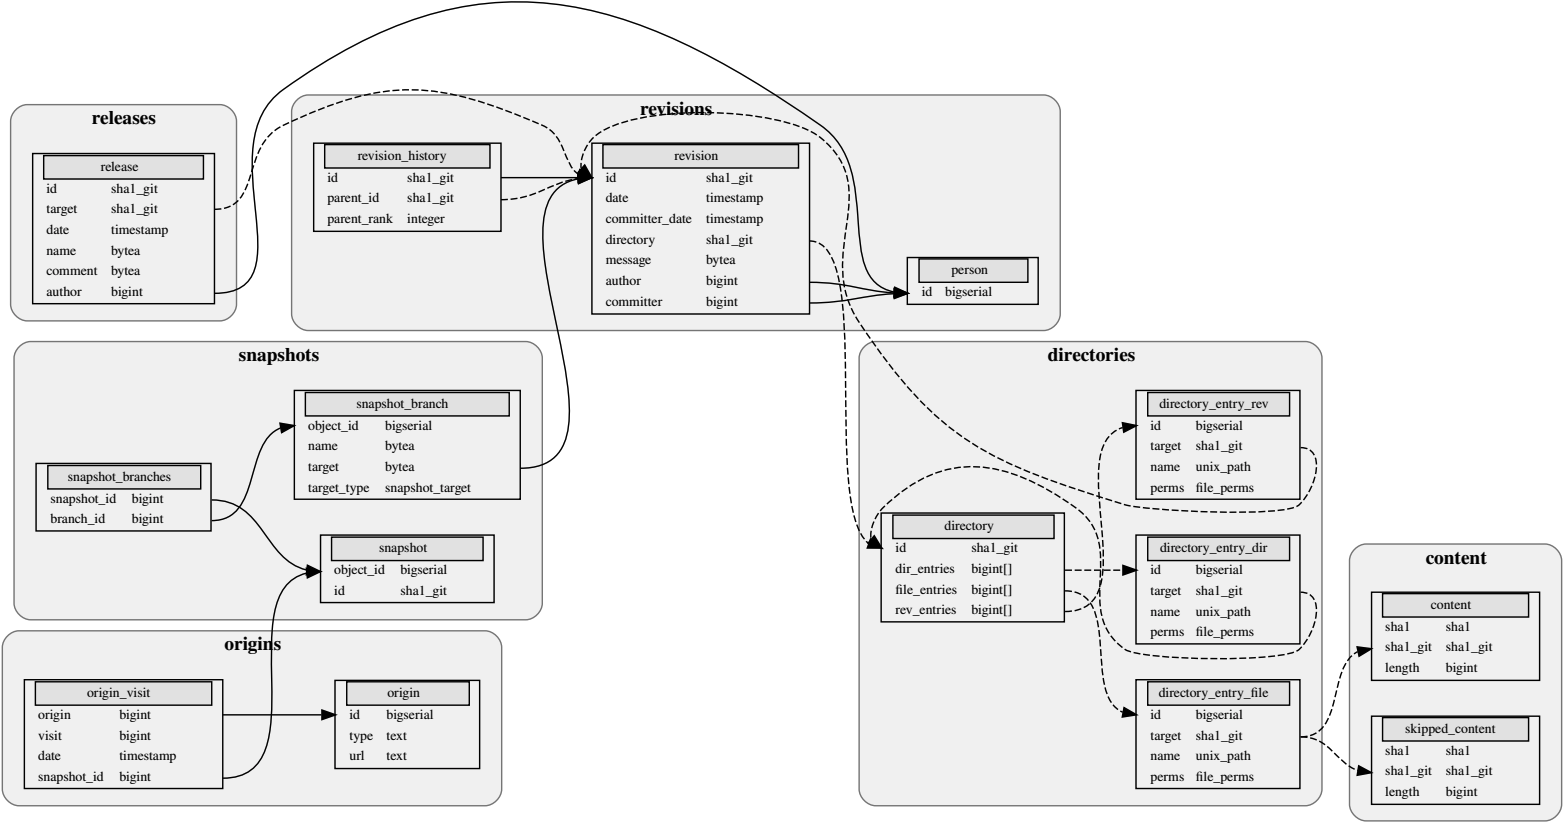
\includegraphics[scale=0.25]{dataset-schema.png}
% \Description{}
% \caption{The results of running the Cox Proportional hazards tool on the data. \keanu{we definitely want better descriptions for the images} \derek{I don't think that we really need the schema in the paper}}
% \label{fig:Schema}
% \end{figure}

\section{Methods}

Most of the work done in this study has been documented in a repository for the benefit of the reader.
References to the repository and the data set used \keanu{and more?} can be found in appendix A below.
\keanu{define artifacts?}

\subsection{Replication}

The first step in the replication was to obtain the data set and gain a proper understanding of it.
A postgreSQL server was created and the data was imported following the tutorial provided by the Software Heritage organization \cite{SQLdataset}.
The data set includes a load.sql file which creates the database according the the schema diagram mentioned in the \emph{Data} section of this paper.
After analyzing this database, queries were created in order to join the necessary tables and extract the relevant values.
The queries accomplish the following objectives: they group records by the url field of the origin table (used to identify projects), filter records to be within the desired timeframe of May 9, 2005 to Jan. 1, 2018, count distinct authors that have participated in a given project, record the host service (depicted by the type field of the origin table), record the earliest and latest revisions associated with each project url, and
\keanu{should we show pseudocode of one of the queries?}

Inside of the repository there is a jupyter notebook (Analysis&Data/data-collection.ipynb).
This notebook used popular python libraries such as psycopg2, pandas, numpy, and matplotlib to connect to the database, extract the results of the previously mentioned queries, manipulate and filter the data, calculate new fields, and plot results.

Constructing additional fields (multi\_repo and duration) using pandas in python. Sort by duration and plot project from start to end month to recreate figure 1.

Perform frequentist analysis on data using survival package in R. First apply kaplan meier based on each attribute, then run Cox proportional hazards tool on the data.

\subsection{Bayesian Survival Analysis}

A common distribution for survival analysis is the exponential distribution \cite{kelter2020bayesian, rethinking}.
\keanu{I don't have anything to write for this}

\section{Results}

\subsection{Replication}

We found the results of our replication study to be extremely similar to those shown in the original paper.

\keanu{Put images here}
\begin{figure}[h]
\centering
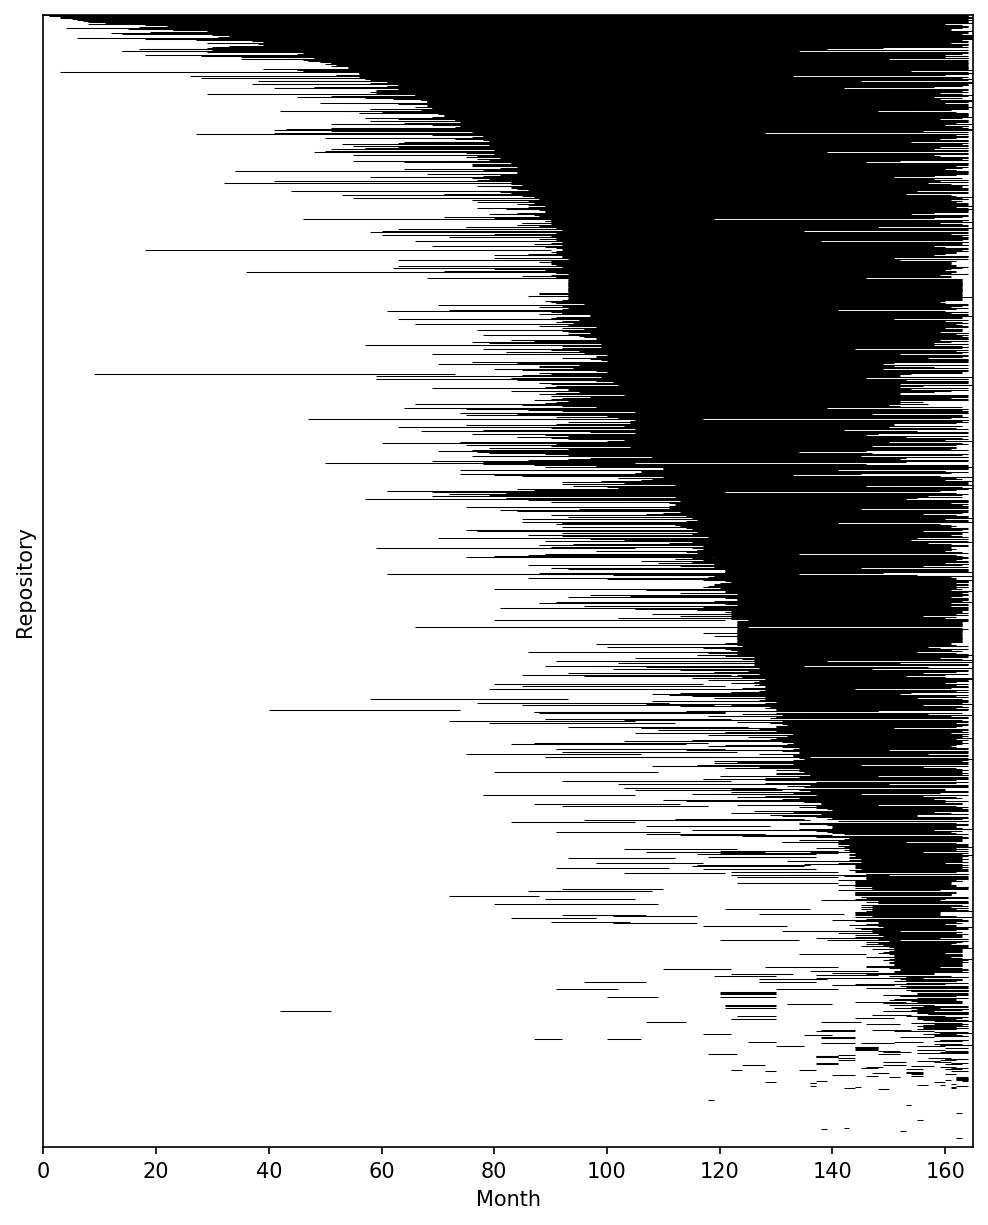
\includegraphics[scale=0.5]{figure1.jpg}
\Description{}
\caption{Graph of project timelines within the given time frame. The projects are ordered by duration.}
\label{fig:figure-1}
\end{figure}

\begin{figure*}[h]
    \centering
    \begin{subfigure}
        \centering
        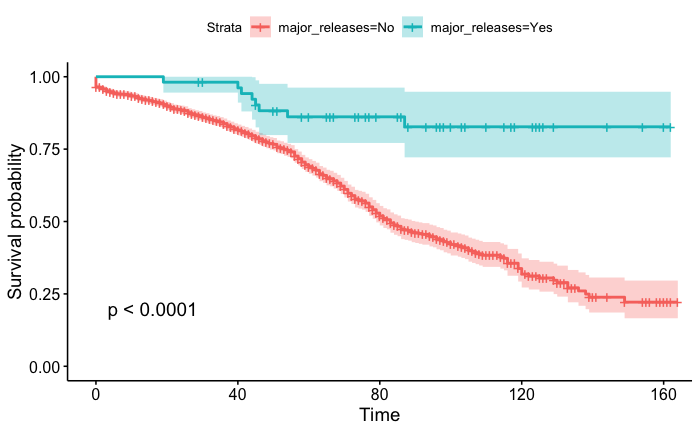
\includegraphics[width=0.45\textwidth]{major-releases.png}   
        \label{fig:major releases}
    \end{subfigure}
    \begin{subfigure}
        \centering 
        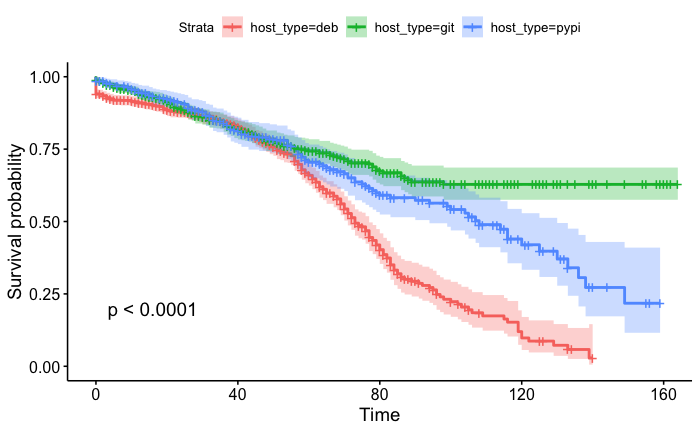
\includegraphics[width=0.45\textwidth]{host_type.png}
        \label{fig:host type}
    \end{subfigure}
    \vskip\baselineskip
    \begin{subfigure} 
        \centering 
        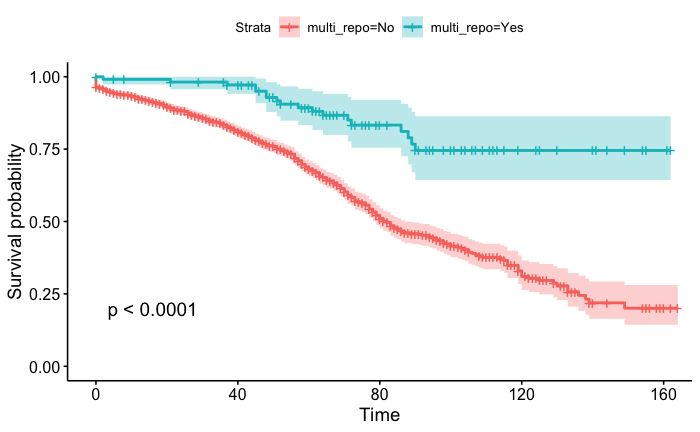
\includegraphics[width=0.45\textwidth]{multi_repo.png}
        \label{fig:multi repo}
    \end{subfigure}
    \begin{subfigure}   
        \centering 
        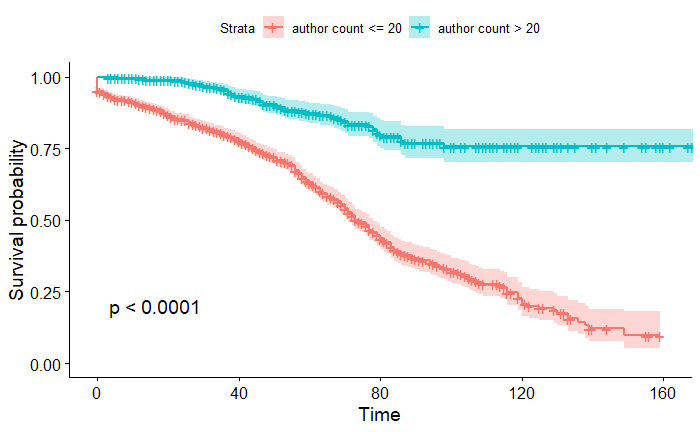
\includegraphics[width=0.45\textwidth]{img/author_count.png} 
        \label{fig:author count}
    \end{subfigure}
    \caption
    {\small KM curves of the python project data analyzed by major releases, host type, multiple repository hosting, and number of authors} 
    \label{fig:KM curves}
\end{figure*}

\begin{figure}[h]
\centering
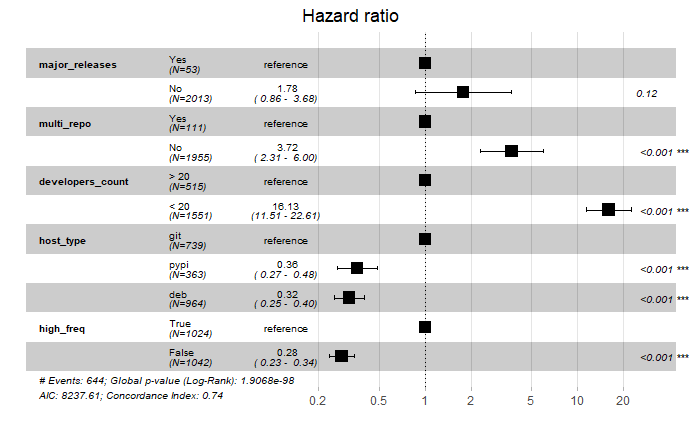
\includegraphics[scale=0.75]{cox-ratios.png}
\Description{}
\caption{The results of running the Cox Proportional hazards tool on the data. \keanu{we definitely want better descriptions for the images}}
\label{fig:Cox}
\end{figure}

\keanu{talk about significance and meaning of the KM and Cox results}

\keanu{As you can see in the Cox table summary, the numbers in each category are slightly different than the original study,
 we plan to look further into what has caused this difference in values}

\subsection{Bayesian Survival Analysis}

\keanu{Nothing for this yet}

\section{Discussion}

\subsection{Comparison of Analyses}

\subsection{Limitations}

\subsubsection{Limitations of the Methods}

The method Ali \emph{et al.} used for censoring was slightly ambiguous.

\subsubsection{Limitations of the Data}

There are inherent differences in the ways developers use the different hosting services \keanu{I have a strong intuition that this is the case, it looks like PyPi and debian don't have as much granularity compared to git and only show major releases, but I don't have anything to back this up, so maybe we can find something to cite for that}. This may skew the results because it may be the case that services such as PyPi and Debian are primarily used to host major releases of a product. This may hide information about the number of developers and the commit frequency.

It may also be worth noting that this data is only for Python projects and that it is possible that different behaviours are associated with development in different languages.
Python is a relatively easy language to use, and can often be used for small tasks that are not maintained.
However, because this data set comprises popular projects, it is unlikely to contain projects that were used for a small task and discarded.

There was no clear method for determining whether a project was hosted in multiple repositories.
The only unique identifier for each project was a url, from which the project name was extracted using regular expressions.
This may have resulted in the extraction of inconsistent project names across host types.
The assumption is that each project that was hosted on multiple repositories would be given the exact same name, and that projects of the same name hosted on different services were indeed the same project (which may not always be the case).
Additionally, it is possible for users on Github to give their projects the exact same name as pre-existing projects created by other users.
However, this issue was accounted for in our analysis, but it is unclear whether Ali \emph{et al.} accounted for this.

The data contains a large portion of censored data.
This means that we did not observe the abandonment of most of the projects.
As data points are censored (denoted by the vertical tick marks in the KM curves), we have a smaller and smaller group of data points to study.
This means that the results towards the 165 month mark may be less representative.
This is to be expected with any SE study, as recent years have lead to an exponential increase in the number of OSS projects \keanu{find citation?}.


The data set contained many revisions (over 4 million) that were not associated with project URLs.
It is unclear how this happened.

\subsubsection{Replication Challenges}

\subsection{Future Work}

Increase the time frame of the study (the original paper could not do this because the paper was written in 2018).

Perform separate studies on each hosting service to remove variability in the way the services are utilized.

\section{Conclusion}

%%
%% The next two lines define the bibliography style to be used, and
%% the bibliography file.
\bibliographystyle{ACM-Reference-Format}
\bibliography{refs.bib}

%%
%% If your work has an appendix, this is the place to put it.
\appendix

\section{Artifacts}
Project Repository: \url{https://github.com/DerekRobin/CSC578B-Project}

Data Set: \url{https://annex.softwareheritage.org/public/dataset/graph/latest/popular-3k-python/sql/}

\end{document}
\endinput
%%
%% End of file `sample-manuscript.tex'.